\documentclass[a4paper, 12pt, oneside]{scrbook}
\usepackage[hyphens,spaces,obeyspaces]{url}
\usepackage[sorting = none, backend=bibtex]{biblatex}
\usepackage[english]{babel}
\usepackage[T1]{fontenc}
\usepackage[utf8]{inputenc}
\usepackage[hidelinks]{hyperref}
\usepackage{graphicx}
\usepackage{subcaption}
\usepackage{epstopdf}
\usepackage{lmodern}
\usepackage{float}
\usepackage{acronym}
\usepackage{booktabs}
\usepackage{caption}
\usepackage{csquotes}
\usepackage{enumitem}
\usepackage{fancyhdr}
\usepackage{url}
\usepackage{listings}
\usepackage[table]{xcolor}
\usepackage{wrapfig}
\usepackage{forest}
\usepackage{tabularx}
\usepackage{colortbl}
\usepackage{booktabs}
\usepackage[onehalfspacing]{setspace}
\usepackage{amsmath}
\usepackage{threeparttable}
\usepackage[english]{cleveref}
\usepackage{listings}
\renewcommand*{\headfont}{\normalfont}
\renewcommand*{\multicitedelim}{\addsemicolon\space}
\renewcommand*{\headrulewidth}{0pt}
\renewcommand*{\arraystretch}{1.5}
\setlength{\parskip}{1.5ex}
\makeatletter
% define new boolean conditional switch for whether
% the abstract is being typeset
\newif\ifabstract
% redefine `\chapter` so it only starts a new page if not typesetting
% the abstract; sets abstract conditional to false after doing so
\renewcommand\chapter{\ifabstract\relax\else%
	\if@openright\cleardoublepage\else\clearpage\fi%
	\fi
	\abstractfalse%
	\thispagestyle{plain}%
	\global\@topnum\z@
	\@afterindentfalse
	\secdef\@chapter\@schapter}

% command for putting the title and name above the abstract; switches
% abstact boolean to true for next `\chapter*` command...
\newcommand{\conclusion}{
	\if@openright\cleardoublepage\else\clearpage\fi
		\begin{center}
			\textbf{\larger{Summary}}\par
			\emph{Hier kommt nach der Fertigstellung der Arbeit noch eine Zusammenfassung der Arbeit mit ein oder mehreren Sätzen hin. Hier kommt nach der Fertigstellung der Arbeit noch eine Zusammenfassung der Arbeit mit ein oder mehreren Sätzen hin. Hier kommt nach der Fertigstellung der Arbeit noch eine Zusammenfassung der Arbeit mit ein oder mehreren Sätzen hin2. }\par
		\end{center}

	\abstracttrue}
\makeatother
\lstset
{
         basicstyle=\footnotesize\ttfamily,
         numbers=left,               	% Ort der Zeilennummern
         numberstyle=\tiny,          	% Stil der Zeilennummern
%         stepnumber=2,               	% Abstand zwischen den Zeilennummern
         numbersep=5pt,              	% Abstand der Nummern zum Text
         tabsize=2,                  	% Groesse von Tabs
         extendedchars=true,
         breaklines=true,            	% Zeilen werden Umgebrochen
         keywordstyle=\color{red},
            frame=b,
 %        keywordstyle=[1]\textbf,    	% Stil der Keywords
 %        keywordstyle=[2]\textbf,
 %        keywordstyle=[3]\textbf,
 %        keywordstyle=[4]\textbf, \sqrt{\sqrt{}}
         stringstyle=\color{white}\ttfamily,
         showspaces=false,
         showtabs=false,
         xleftmargin=27pt,
         framexleftmargin=27pt,
         framexrightmargin=5pt,
         framexbottommargin=4pt,
%         backgroundcolor=\color{lightgray},
         showstringspaces=false      	% Leerzeichen in Strings anzeigen ?
}
\addbibresource{bibliography.bib}

\begin{document}
	\frontmatter
	
\def\title{Titel-TODO}
\def\abgabe{xx.xx.2023}

\begin{titlepage}
	
	
	
	\vspace{5pt}
	
	\begin{center}
		
		\Large \textbf\title
		
		\vspace{50pt}
		
		\large Studienarbeit T3\_3101
		
		von 
		
		\large \textbf{Rico Kursidem} 
		
		\vspace{15pt}
		
		im
		
		\large Studiengang Angewandte Informatik
		
		an der Dualen Hochschule Baden-Württemberg Mosbach

        \vspace{10pt}

        
\includegraphics[height=3.5cm]{images/dhbw-logo.jpg}
		
		\vspace{20pt}
		
		\large Abgegeben am: \abgabe
		
		\vspace{30pt}

		
		\begin{table}[h]
			\centering
			\begin{tabular}{r l}
				\large\textbf{Matrikelnummer, Kurs} & \large 5451998, MOS-INF20B \\
                \large\textbf{Betreuer der Dualen Hochschule} & \large Philipp Abele \\
			\end{tabular}
			
		\end{table}
		
	\end{center}
	
	
\end{titlepage}
	\chapter*{Abbreviation} 
\begin{acronym}
	%A
	%B
	%C
	%D
	%E
	\acro{EDA}{Exploratory Data Analysis}
	%F
	%G
	%H
	%I
	\acro{IDA}{Initial Data Analysis}
	%J
	%K
	%L
	%M
	%N
	%O
	%P
	%Q
	%R
	%S
	%T
	%U
	%V
	%W
	%X
	%Y
	%Z
\end{acronym}
	\tableofcontents
	\listoffigures
	%\listoftables
	%\lstlistoflistings
	\nocite{*}

	\mainmatter

	\pagebreak
%	\conclusion
	\chapter{Introduction} 
	
	\chapter{Theoretical Basis}
	
		\section{Exploratory Data Analysis} \label{EDA}
			
			\noindent Frederik Hardwig describes Exploratory Data Analysis (\ac{EDA}) as two thinks. As a Way of Thinking and a Method to work with data. 
			The Data Miner should always keep in mind, that you need to look for new Patterns that weren't expected, because they are the most interesting. It is important not trying to proof your own Thesis from before the Analyzing Process but to find new ones and always keep open to new findings. Also the Data Analyst should be skeptic towards Methods that compromise Data. If Data is summarized there will always be some loss of Information and the Hypothesis that will be based on these results will be not complete. To avoid this it is a good thing being skeptic towards compressed data. 
			As a Method, \ac{EDA} works with a lot of visualization to find patterns in Datasets. It is important not to confuse Data Analysis and Statistics. It is important to keep in mind that even the most used statistical Methods could have some hidden assumptions about the data. It is always suggested to use diagrams and other visual methods to display data to minimize errors resulting out of these assumptions.\cite{Hardwig:Explortory_Data_Analysis}
			
			\noindent \ac{EDA} tries to generate a understanding of the data and not to proof already stated Hypothesis. This contrasts the Initial Data Analysis (\ac{IDA}) where it is more common to look closely for findings that are needed to develop a modal and testing hypothesis. The goals of \ac{EDA} is to develop and evaluate Hypothesis, provide recommendations for statistical Techniques to support the analysing process and provide Methods to collect more Data. It tries to find relationships between elements and get the main features of the data. 
			
			\noindent To achieve these goals it uses different Methods. Descriptive Statistics is used to get a overview of the Data and the structure of the data. It is very important to get a feeling for the data structure to get the most meaningful and efficient results. In \ref{fig:statistical_description} we can see the main statistical characteristics of a dataset, witch contains the top female chess players in the world by the Rating in Standard Chess games. We can see the number of fields, that are filled (count), the median of the value(mean) and the standard deviation(std). It also shows us the Maximum (max) and minimum (min) and the higher, lower and middle quantil (25\%, 75\%, 50\%).
			
			\begin{figure} [H]
				\centering
				\resizebox{\linewidth} {!} {
					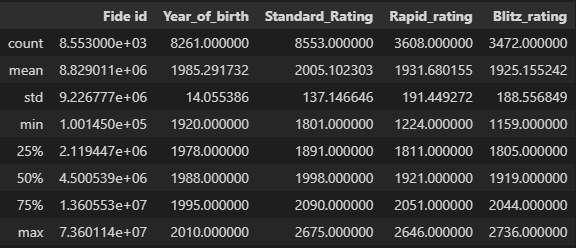
\includegraphics{res/df_describes.png}
					
				}
				\caption{statistical description of the data}
				\label{fig:statistical_description}
			\end{figure}
		
			\noindent To visualize these statistical Properties we can use a Box-Plot. In \ref{fig:boxplot} is the standard rating column of the data visualized. This method can also applied on all columns with a metric datatype. So we could do the same with the other rating fields and the year of birth, but the id doesn't make sense because it is a nominal field. 
			
			\begin{figure} [H]
				\centering
				\resizebox{\linewidth} {!} {
					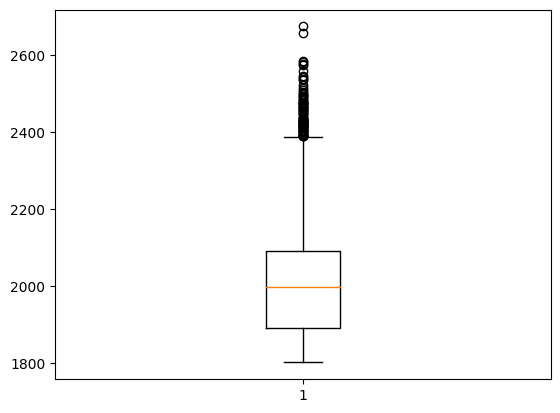
\includegraphics{res/boxplot.png}
					
				}
				\caption{Box-Plot of the standard rating}
				\label{fig:boxplot}
			\end{figure}
		
			\noindent An other way to get more information over the data is to group it by nominal fields. In this example we can group the data by federation or title of the chess player. In \ref{fig:groupeby} are the median given grouped by the federation.
			
			\begin{figure} [H]
				\centering
				\resizebox{\linewidth} {!} {
					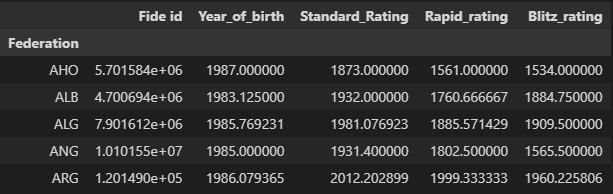
\includegraphics{res/groupby.png}
					
				}
				\caption{Group by the country and showing the median}
				\label{fig:groupeby}
			\end{figure}
			
			To explore the relationships of the fields in the data we need to reduce the dimensions of the data elements. in our case one element has  dimensions. The standard, rapid, blitz rating and also the players age. We need to dissect the four dimensions to two. To do this we plot every single field against every other in their own chart. These charts can be seen in \ref{fig:crosschart}. We can also add a fifth nominal field by coloring the data points according to the Title. The result of the chart matrix is symmetrical and the diagonal charts are the same values plotted against each other so we only need to look at one side of the matrix.
			
			\begin{figure} [H]
				\centering
				\resizebox{\linewidth} {!} {
					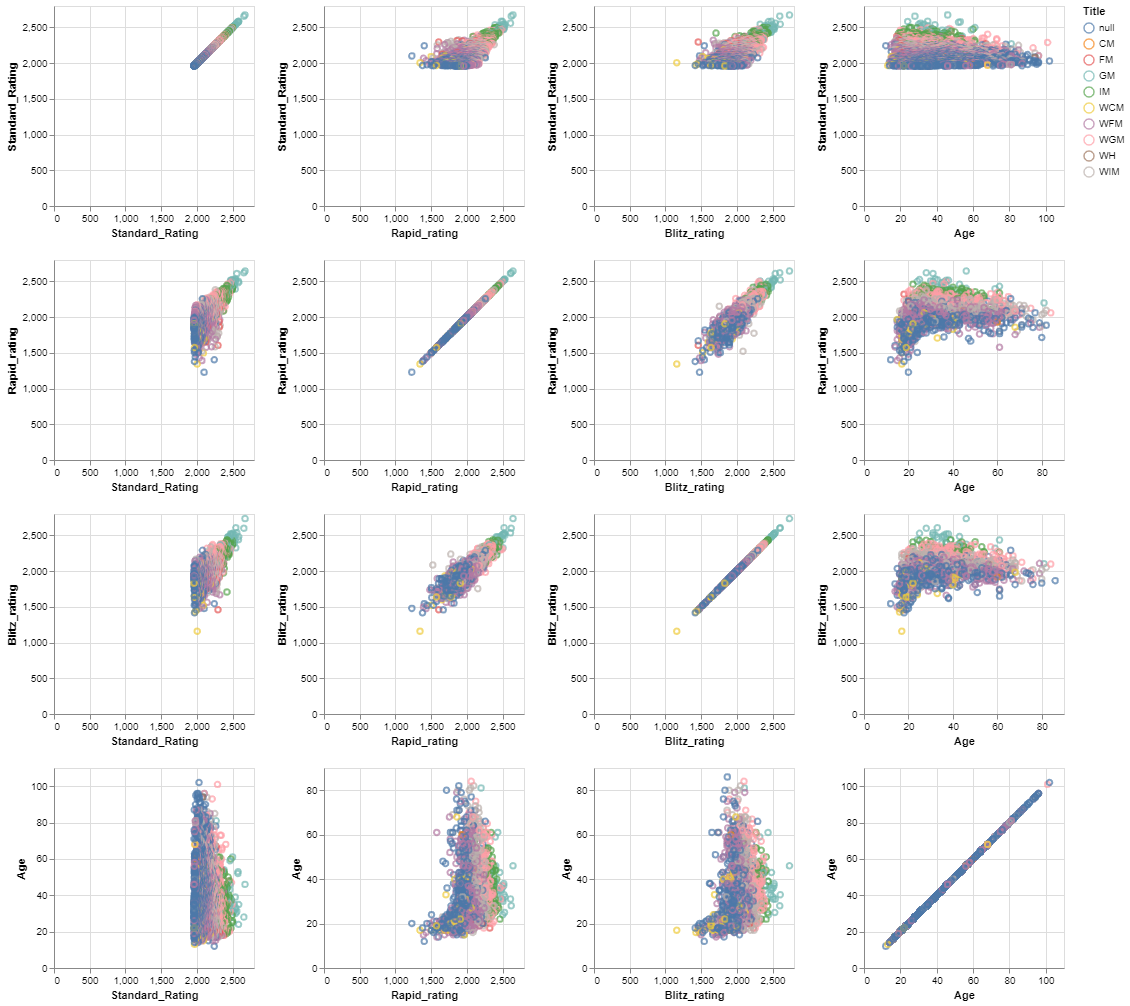
\includegraphics{res/crosschart.png}
					
				}
				\caption{Plotting every data field against each other}
				\label{fig:crosschart}
			\end{figure}
			
			\noindent Out of the Charts in \ref{fig:crosschart} we can also generate the linear Correlation of the fields. The closer to one or minus one the value is, the better the two fields correlate linear. So we can say that in our data, blitz and rapid rating correlate more linear than standard rating with the other both in our data. But there is more to think about in this assumption. The data shows only the Players with a standard rating above 1960 so there is a hard line in the data. This results in a incomplete model of reality and we need to include it into our result. 
			The hypothesis could be that the blitz and rapid ratings correlate linear, with a value of 0.878720, under the top Players with a standard rating above 1960.
			We cannot see non linear correlations in this matrix so we could oversee them.
			
			\begin{figure} [H]
				\centering
				\resizebox{\linewidth} {!} {
					\includegraphics{res/Correlation.png}
					
				}
				\caption{Correlation chart}
				\label{fig:correlation}
			\end{figure}
			
	\chapter{Application}
		\section{First Steps with a Dataset}
		%TODO: beschreiben des ersten kapitels
			\subsection{Exploratory Data Analysis}
			\noindent A dataset is provided with three values. It has data of a shaft-bearing-system loaded with rotational force and rotations per minute and a third value, which is the lifetime in hours.
			
			\begin{figure}[H]
				\centering
				\begin{minipage}[b]{0.4\textwidth}
					\resizebox{\linewidth} {!} {
						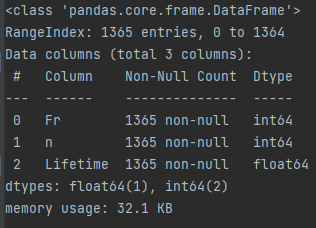
\includegraphics{res/firstEDA/df_info.png}
					}	
					\caption{df.info()}
					\label{fig:EDA_info}
				\end{minipage}
				\hfill
				\begin{minipage}[b]{0.4\textwidth}
					\resizebox{\linewidth} {!} {
						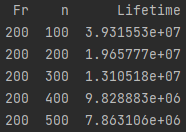
\includegraphics{res/firstEDA/df_head.png}
					}	
					\caption{First 5 Datapoints in the table}
					\label{fig:EDA_head}
				\end{minipage}
			\end{figure}
			
			\noindent After showing the info of the data and getting a general feel for the data set, we can see how the data points are related to each other with the same techniques from Chapter \ref{EDA}. We create a chart for every feature of a data point and get the charts in picture \ref{fig:EDA_crossplot}. the charts where we use \textit{Fr} and \textit{n} aren't correlated at all. If we zoom in more we can see that the points are evenly distributed. This makes sense if the data is a systematic test, with the changing parameters of rotation n and radial Force Fr. In picture \ref{fig:EDA_3Dscatter} there is a 3D scatter of the data points with n and Fr on the x and y axis and the Logarithm of the Lifetime on the z axis. It shows a better Picture of the data were the equal distributed points show a good visible plane. The lifetime increases rapidly when n and Fr go towards zero and shrink exponential when one of both parameters are increased.
	
			\begin{figure}[H]
				\centering
				\begin{minipage}[b]{1\textwidth}
					\resizebox{\linewidth} {!} {
						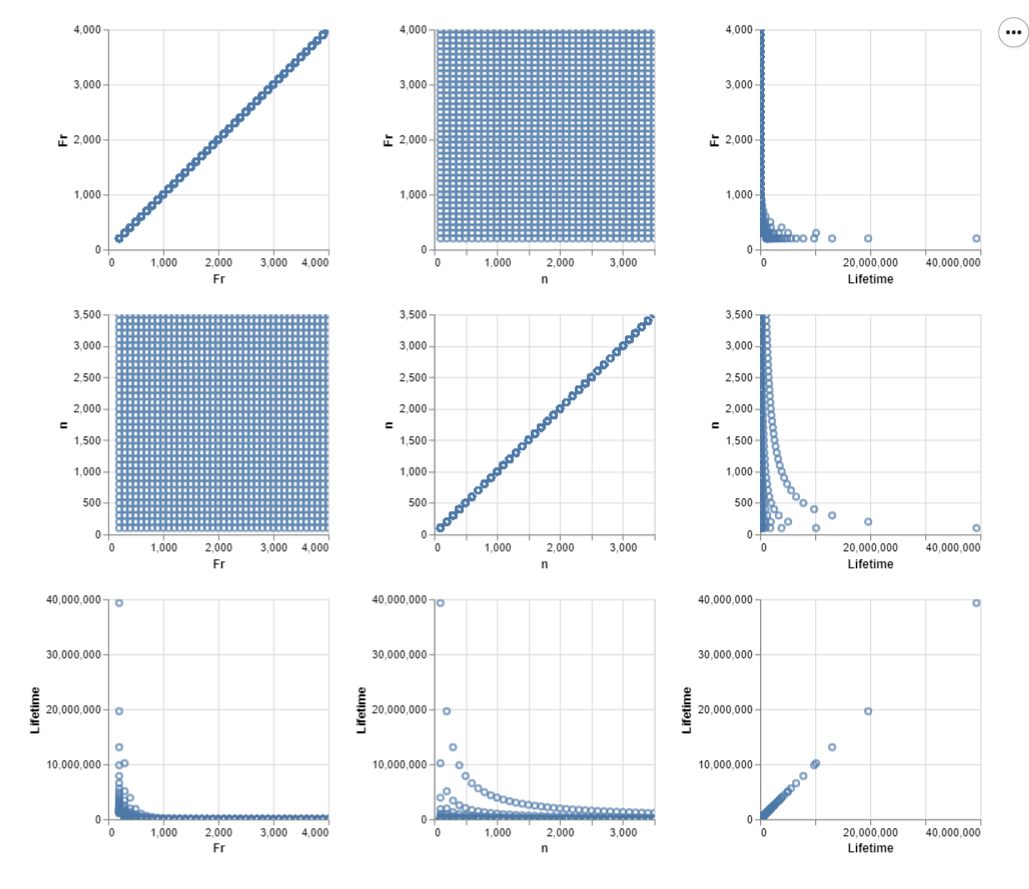
\includegraphics{res/firstEDA/crosschart.png}
					}	
					\caption{All Data fields plotted against each other}
					\label{fig:EDA_crossplot}
				\end{minipage}
				\hfill
				\begin{minipage}[b]{1\textwidth}
					\resizebox{\linewidth} {!} {
						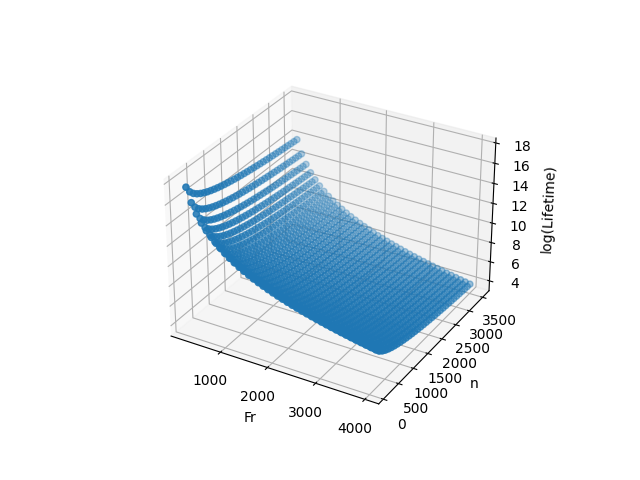
\includegraphics{res/firstEDA/3dscatter.png}
					}
					\caption{3D scatter of the Data set}
					\label{fig:EDA_3Dscatter}
				\end{minipage}
			\end{figure}
		
			\subsection{Machine Learning Model}
				\noindent After the analytic exploration of the data set, we can train our first machine learning model on the data. My goal is to use the Rotation n and the Force Fr as input and get the Years of Life as the output. For this we first need to load the data from the csv and create a feature data class out of it, with which the machine learning model can work with. For this I implemented the \texttt{FeatureDataclass} to hold the test and training data. In Picture \ref{fig:FeatureDataclass} is the Code for this class. In the Constructor of the class the given data frame is cut into the input and output values and saved into \texttt{self.sample} and \texttt{self.label}. Beside the Constructor also \texttt{\_\_len\_\_} and \texttt{\_\_getitem\_\_} is added. These methods return the length of the data set or the element at the given index.
				
				\begin{figure} [H]
					\centering
					\resizebox{\linewidth} {!} {
						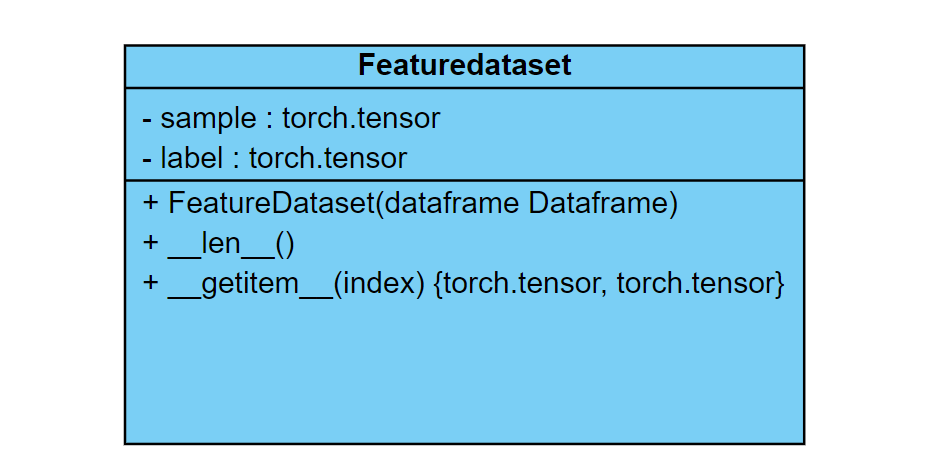
\includegraphics{res/firstEDA/feature_dataset.png}
						
					}
					\caption{FeatureDataset class}
					\label{fig:FeatureDataclass}
				\end{figure}
				
				\noindent In the main class the Lifetime column in the data is classified into years. This is achieved by converting the hours to years and rounding down. After the data is as it need to be, two FeatureDataset objects are created. One to train the model on and the other to test it. To feed the data to the model, it needs to get divided into small batches. Data loaders provide this functionality so one for the testing- and for the training data are created. I used a batch size of 10 after some testing because it fitted very well with the overall size of the data set.
				
				\noindent Before the training can start, a Model must be created. I decided I want to keep the Network simple, so I only used two ReLU-Layers with 10 nodes each. The Input layer has two nodes, corresponding with the two input variables. The Export layer has 6 Nodes, each representing one class of the labels. In Picture \ref{fig:layer_first} the layers are shown. 
				
				\begin{figure} [H]
					\centering
					\resizebox{\linewidth} {!} {
						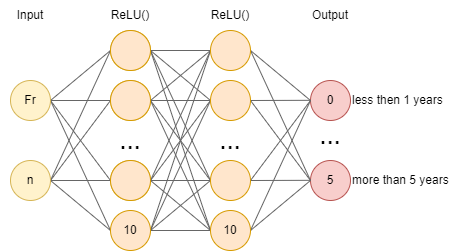
\includegraphics{res/firstEDA/layer_model.png}
						
					}
					\caption{Layers of the first machine learning model}
					\label{fig:layer_first}
				\end{figure}
			
				\noindent The parameters for this program is a learning rate of $1 * 10^{-7}$, the amount the model modifies its weights an biases. I tried different epochs, how often the optimization loop is done, and stick with 200 because it fits well with the learning rate. After all the parameters are set, the training can begin. 
				
				\noindent In every epoch the program does a training and a testing loop. In the training loop the model gets trained on the data. The model gets small batches of data from the data loader and optimizes its weights and biases every step using the optimizer function. In this case I use a cross entropy loss function. It uses the probability output of the model to determine a distance to the desired output and adjusts the weights in every iteration. This function is well suited to classification problems. After the model is trained, it gets tested on the testing data. Here the program does not modify its weights anymore and just computes the loss and accuracy of the model. This Values describe the difference between the models prediction and the test data. The lower the loss, the better. The higher the accuracy, the better. 
				
				\noindent after all the epochs are done, the accuracy and loss values are plotted on a diagram using \texttt{matplotlib}. In Picture \ref{fig:lossAndAccuracy} these diagrams are shown after an training of 200 epochs.
				
				\begin{figure} [H]
					\centering
					\resizebox{\linewidth} {!} {
						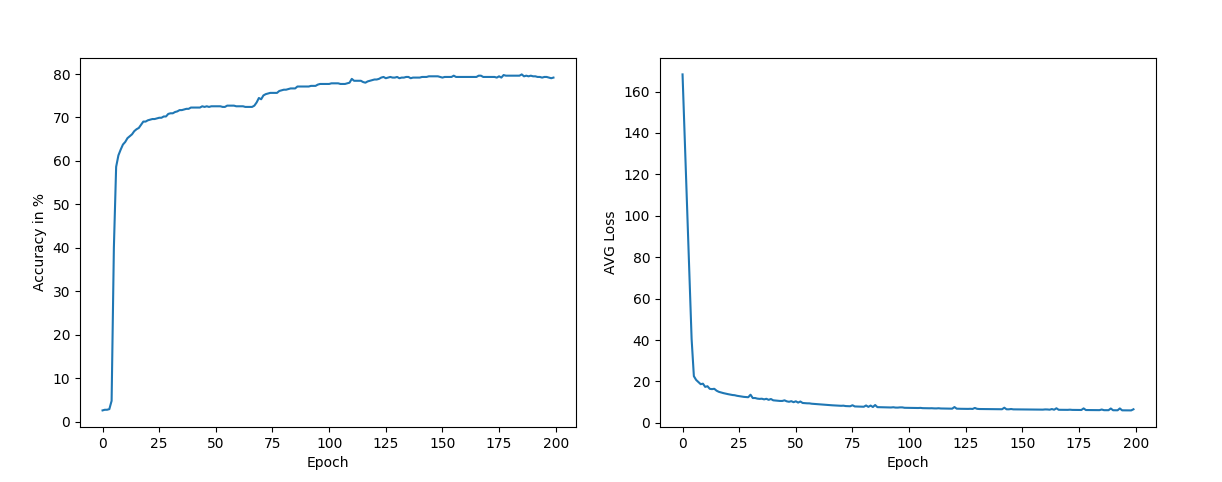
\includegraphics{res/firstEDA/lossAndAccuracy.png}
						
					}
					\caption{Loss and Accuracy over 200 epochs}
					\label{fig:lossAndAccuracy}
				\end{figure}
			
			\subsection{Parameter Study}
			
				\noindent A parameter study is a way to find the best parameters for the machine learning model and the data. Some parameters will be chosen an varied isolated from each other to se the effect of them. It also gives insights on what are the extremes of these valued and where the best values lay. In this first parameter study the Learning rate of the model, the batch size of the training data and the epochs will be varied. 
				
				\noindent Before the parameter study starts, the standard valued need to be defined. After these Values are defined I will only change one so the effects of every variable can be isolated. 
				\begin{gather}
					learning\_rate = 1e^{-6}\\
					batch\_size = 20\\
					epochs = 200
				\end{gather}
				
				\subsubsection{learning rate}
					The learning rate is the value that regulates the changes the model does to its weights and biases. In Picture \ref{fig:parameter_study_learning} are two diagrams showing the Accuracy and the average loss of the machine learning model over epochs. It has multiple learning processes shown for different learning rates. It is visible that the larger learning rates are not as smooth as the smaller ones. The Accuracy jumps between high and low values because the model makes too huge changes after every optimization. the smaller the learning rates get, the smoother the graphs get. But if the learning rates gets to small, it can hinder the learning process because the model doesn't modify its weights enough to change its own behavior. In the left of the diagram \ref{fig:parameter_study_learning} the average loss over the epochs is shown. The Model that learned with the larger learning rate does not minimize its loss because it doesn't change its behavior in a significant amount. The lower the learning rate, the better the model minimizes its loss and even if the Accuracy jumps very hard, the average loss is very low and constant.
					
					\begin{figure} [H]
						\centering
						\resizebox{\linewidth} {!} {
							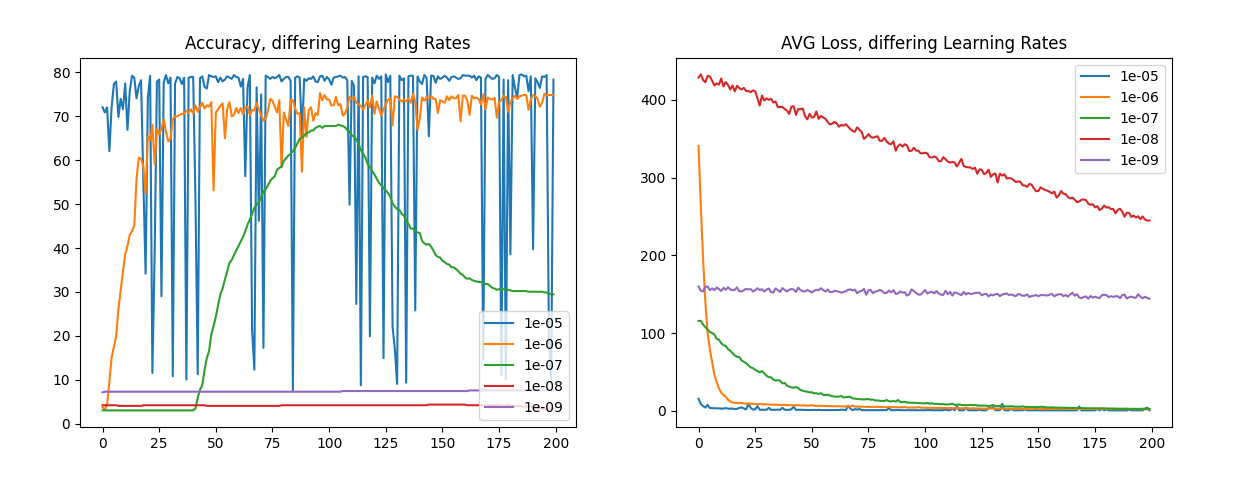
\includegraphics{res/parameter_study/learning_ps.png}
							
						}
						\caption{Accuracy and loss for different learning rates}
						\label{fig:parameter_study_learning}
					\end{figure}
					
				\subsubsection{batch size}
					\noindent The size of the batched describes the size of samples the Model gets to train and learn. If the batch size is changed the model refines it learning process to more or less data depending the size. In the Diagram \ref{fig:parameter_study_batch} the model run for six different batch sizes. The accuracy is only good, if the size is not too huge or small. Accuracy with batch size 10 and 100 is not as good as with the sized between. The best result is with 50 where the Accuracy does not jump as much as with 20, 30, or 40. The average Loss is quite similar with all batch sizes. In the right Diagram in picture \ref{fig:parameter_study_batch} the average loss for the different batch sizes are shown. 
					
					\begin{figure} [H]
						\centering
						\resizebox{\linewidth} {!} {
							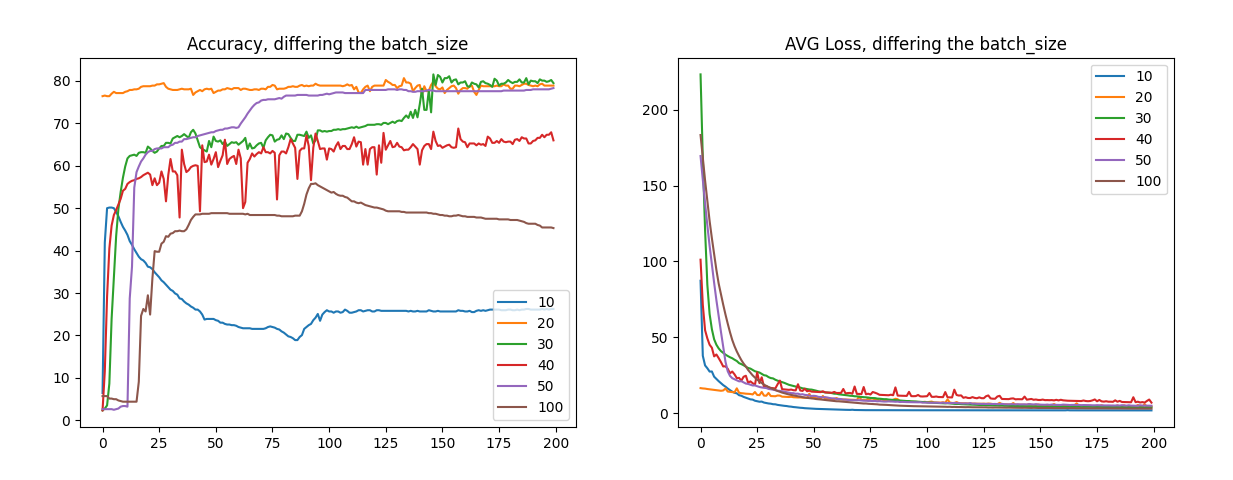
\includegraphics{res/parameter_study/batch_ps.png}
							
						}
						\caption{Accuracy and loss for different batch sizes}
						\label{fig:parameter_study_batch}
					\end{figure}
					
					
				\subsubsection{epochs}
					In the parameter study for epochs, I changed the value of the learning rate to $1e^{-8}$ so the difference in the results can be seen better. If we change the epochs of the model it has less iterations to optimize its weights and biases. So in theory the more epochs the nearer is the model to its potential. In this test, shown in Table \ref{tab:parameter_study}, the accuracy of the model was at its maximum around 75\%. In the first two runs the Model did not had the time to reach a very high accuracy, but after 100 epochs the model could reach the 70\% mark quite often. 
				\begin{table}[!h]
					\begin{center}
						\begin{tabular}{| c || c | c | c | c  | c | c | }
							\hline
							Epochs & 10 & 50  & 100 & 200 & 500 & 1000 \\
							\hline
							Accuracy & 17.7419  & 45.8944 & 75.5131 & 75.6598 & 52.4926 & 71.5543 \\ 
							\hline
						\end{tabular}
						\caption{\label{tab:parameter_study}The Accuracy of the different epochs}
					\end{center}
				\end{table}	
	 
	\chapter{Implementation}
		
		\section{Parameterstudy with AutoPyTorch}
		
		\noindent The goal of this work is to realise an environment, where a Parameter study is performed automatically. For this purpose the AutoPyTorch library is used. Since it needs ubuntu to run, it will run in an Docker Container with the ubuntu Image as base and will clone the repository and install all Dependencies needed to run a automatic Parameter study.
		
		\subsection{Dockerfile}
		
		\noindent Docker is a technology that creates run environments for Applications. These containers are lightweight and easy to start, stop and pause. To run a Ubuntu Container with AutoPyTorch in it, a Dockerfile needs to be run and started on Docker Desktop, the Docker Engine for Windows Desktop PCs.
		
		\noindent This Dockerfile will start on a Ubuntu foundation, install GitHub and AutoPyTorch and all the dependencies. After that the GitHub repository of this Project will be cloned for further development inside of the container. 
		
		\noindent In the first 10 lines of the Dockerfile the base image is set to ubuntu:latest and some Arguments are defined. These Arguments are set when starting the container by the compose file or with the \textit{docker run} command. they will be important later in the file. 
		
		%TODO: beautify the code or leave it
		
		\noindent \lstinputlisting[firstline=1, lastline=10]{res/code/Dockerfile}
		
		\noindent In the following lines zsh is installed to make the command-line of the container look better. Also the Linux packages git, gpg and curl are installed and updated. All these three are needed to communicate with the docker container and getting the GitHub repository cloned.
		
		\noindent \lstinputlisting[firstnumber=12, firstline=12, lastline=20]{res/code/Dockerfile}
		
		\noindent The following code block is installing the GitHub CLI, clones the repository with the autoPyTorch in it and sets up a authentication process for GitHub. The data is taken from the arguments before. All arguments are explained in the Docker Compose section. After the GitHub environment is setup, the correct branch is checked out. 
		
		\noindent \lstinputlisting[firstnumber=22, firstline=22, lastline=45]{res/code/Dockerfile}
		
		\noindent The ubuntu system is updated and the autoPyTorch library is installed. Before the pip install command can be executed, python, pip and some other dependencies are installed. This part of the Dockerfile can be found on the autoPyTorch Repository (https://github.com/automl/Auto-PyTorch/blob/master/Dockerfile). 
		
		\noindent Because this is in a Docker environment some extra dependencies are reqired. In line 67 and 68 libgl1 and libglib2.0.0 are installed. 
		
		\noindent \lstinputlisting[firstnumber=48, firstline=48, lastline=68]{res/code/Dockerfile}
		
		\noindent After the Dockerfile is finished, the container needs to open a CMD so it doesn't stop in impatiently and a Visual Studio Code instance can be attached.
		
		\noindent \lstinputlisting[firstnumber=70, firstline=70, lastline=70]{res/code/Dockerfile}
		
		\subsection{Docker Compose}
		
		%TODO: Compose
		
		Docker provides a possibility to create containers with all the parameters defined in a \textit{.yaml} file. Docker Compose has some extra benefits as well but I will mainly use it as a file where I can save my parameters. 
		
		\noindent This Docker Compose file builds a Container from the Folder it is in. It will create an Image named \textit{ubuntu\_python\_env} and an Container from this Image with the same. It also uses the \textit{tty} parameter to make sure that the container does not terminate after an instant so a Visual Studio Code can be attached. 
		
		\noindent The Arguments given are used in the Dockerfile. 
		
		\begin{itemize}
			\item gh\_token:  Authenticator token from GitHub. 
			\begin{enumerate}
				\item To create this Token, navigate to the GitHub Settings -> Developer Settings -> Personal Access Token
				\item create a classic Token with the following minimum scopes.
				\begin{enumerate}
					\item repo
					\item workflow
					\item read:org
				\end{enumerate}
				\item Copy the generated Token into the docker Compose file
			\end{enumerate}
			\item gh\_email:  E-mail of the Token holder
			\item gh\_uname:  Name of the Token holder
			\item gh\_repo\_owner:  To clone the right Repository.
			\item gh\_rep\_name:  To clone the right Repository.
			\item gh\_branch:  To clone the right Branch. It will be possible to use the main branch, when the pull request is merged.
		\end{itemize}
		
		\noindent \lstinputlisting{res/code/compose.yaml}
		
		%TODO: Github Token
		
		\subsection{Python Script}
	
		%TODO: Explaining Script
	
		\section{Results}
		
		%TODO: Explaining Results of the Script
		
	\chapter{Summary} % Fazit
	
	\frontmatter
	\printbibliography
\end{document}
